

\begin{frame}{Neural Networks -- method summary}

% \maketag{un/SUPERVISED} 
\maketag{regression} \maketag{classification}
\maketag[50]{(non)parametric}
\maketag{BLACK-BOX} \maketag{feature selection}

\medskip

\highlight{General idea}
\begin{itemize}
  \item Learn \textbf{composite function} through series of nonlinear feature 
  transformations, represented as \textbf{neurons}, organized hierarchically 
  in \textbf{layers}
  \begin{itemize}
    \item Basic neuron operation: 1) affine \textbf{transformation} $\phi$ (weighted sum of inputs), 
    % multiplying inputs with weights (possibly including bias term), 
    2) nonlinear \textbf{activation} $\sigma$
    % , applying (nonlinear) function to transformed inputs
    \item Combinations of simple building 
    blocks to create a complex model
  \end{itemize}
  \item Optimize via \textbf{mini-batch stochastic gradient descent (SGD)} variants:
  \begin{itemize}
    \item Gradient of each weight can be infered from the \textbf{computational graph} of the network\\
    $\rightarrow$ \textbf{Automatic Differentiation} (AutoDiff)
    \item Algorithm to compute weight updates based on the loss is called \textbf{Backpropagation}
    %\textbf{Forward pass}: predict result with current parameters and 
    %compute empirical risk 
    %\item \textbf{Backward pass}: update each parameter in proportion to its 
    %error contribution $\Rightarrow$ gradients
  \end{itemize}
\end{itemize}

\medskip
 
\highlight{Hypothesis space} ~~
$\Hspace = \left\{ \fx: \fx = \tau \circ \phi \circ \sigma^{(h)} \circ
\phi^{(h)} \circ \sigma^{(h - 1)} \circ \phi^{(h - 1)} \circ ... \circ 
\sigma^{(1)} \circ \phi^{(1)} (\xv) \right\}$

\smallskip
\begin{center}
\begin{minipage}[b]{0.24\textwidth}
  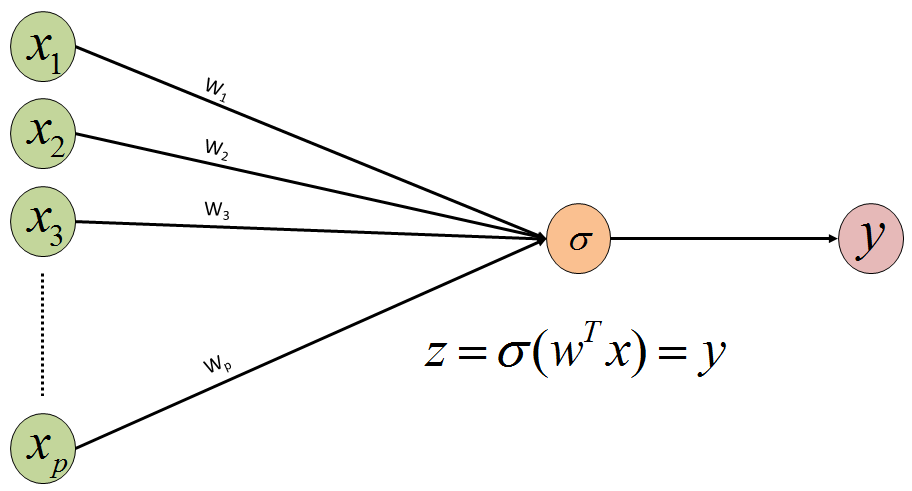
\includegraphics[width=0.9\textwidth]{figure/nn-single-neuron} \\
  %\tiny{Single neuron}
\end{minipage}%
\begin{minipage}[b]{0.24\textwidth}
  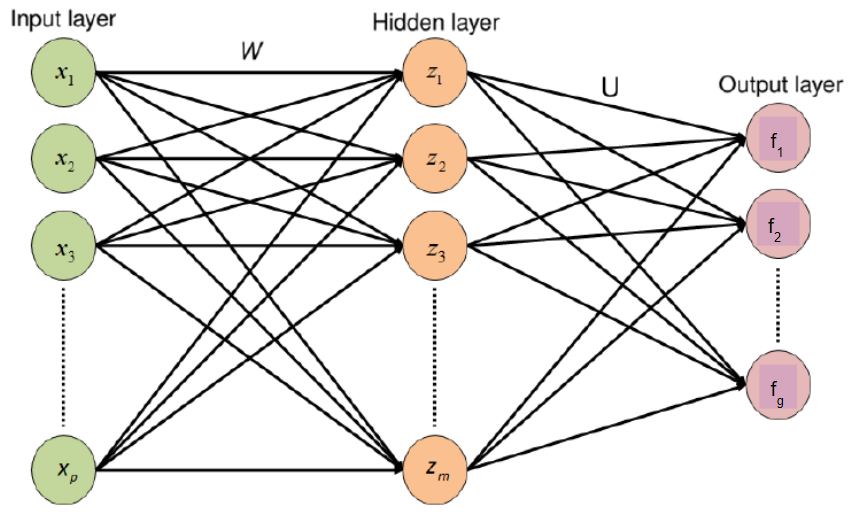
\includegraphics[width=0.9\textwidth]{figure/nn-feedforward} \\
  %\tiny{(Fully-connected) Feedforward network, 1 hidden layer}
\end{minipage}%
\end{center}


\end{frame}

% ------------------------------------------------------------------------------

\begin{frame}{Neural Networks -- method summary}

\footnotesize

\highlight{Architecture}

\begin{itemize}
    \item Input layer: original features $\xv$
    \item Hidden layers: nonlinear transformation of previous layer $\phi^{(h)} = \sigma^{(h - 1)}(\phi^{(h-1)})$
    \item Output layer: number of output neurons and activation depends on problem $\tau(\phi)$
    \begin{itemize}
    \item Regression: one output neuron, $\tau = $ identity
    \item Binary classification: one output neuron, $\tau = \frac{1}{1 + \exp(- \thx)}$ (logistic sigmoid)
    \item Multiclass Classification: $g$ output neurons, $\tau_j = \frac{\exp(f_j)}{\sum_{j=1}^g \exp(f_j)}$ (softmax)
\end{itemize}
\end{itemize}


\highlight{Empirical risk} In general, compatible with any differentiable loss

\medskip

\highlight{Optimization}

\begin{itemize}
  \item Variety of different optimizers, mostly based on some form of 
  \textbf{stochastic gradient descent (SGD)}\\
  \item Improvements: 
    \begin{itemize}
        \item[(1)] Accumulation of previous gradients $\rightarrow$ \textbf{Momentum}
        \item[(2)] Weight specific scaling based on previous squared gradients $\rightarrow$ \textbf{RMSProb}\\
        $\Rightarrow$ \textbf{ADAM} combines (1) and (2) 
        \item[(3)] Learning rate schedules, e.g., decaying or cyclical learning rates
    \end{itemize}
    \item Training progress is measured in full passes over the full training data, called \textbf{epochs}
    \item \textbf{Batch size} is a hyperparameter and limited by input data dimension
  % \item Crucial role of \textbf{regularization} due to high expressivity of 
  % NNs' hypothesis spaces
\end{itemize}

\end{frame}

% ------------------------------------------------------------------------------

\begin{frame}{Neural Networks -- method summary}

\highlight{Network types} ~~ Large variety of architectures for different data modelities
\begin{itemize}
  \item \textbf{Feedforward NNs / multi-layer perceptrons (MLPs):} sequence of 
  \textbf{fully-connected} layers $\Rightarrow$ tabular data
  \item \textbf{Convolutional NNs (CNNs):} sequence of feature map extractors 
  with spatial awareness $\Rightarrow$ images, time series
  \item \textbf{Recurrent NNs (RNNs):} handling of sequential, variable-length 
  information $\Rightarrow$ times series, text, audio
  \item \textbf{Transformers:} Learning invariances from data, handling multiple/any data modalities
  %\item Unsupervised: \textbf{autoencoders}, \textbf{generative adversarial networks (GANs)}, \dots
  % \item \textbf{Autoencoders:} learning unsupervised embeddings
  % \item \textbf{Generative adversarial networks (GANs):} learning to generate 
  % artificial samples
\end{itemize}

\begin{minipage}[b]{0.49\textwidth}
\begin{center}
  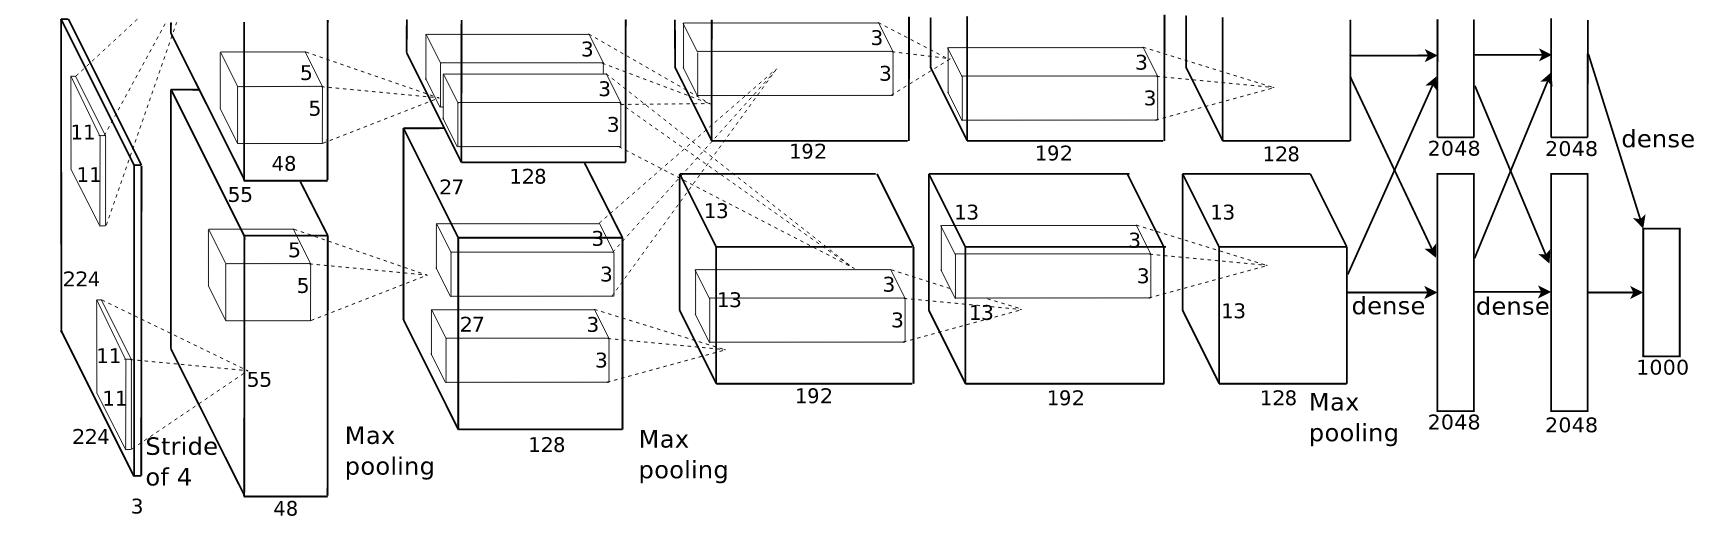
\includegraphics[width=.9\textwidth]{figure/nn-cnn-1} \\
  \tiny{Convolutional network architecture}\\ \medskip
  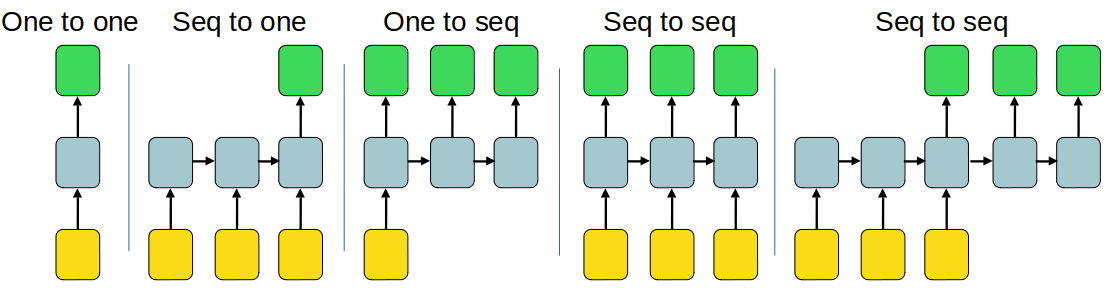
\includegraphics[width=.9\textwidth]{learners-overview/figure/one_to_one.png} \\
  \tiny{Recurrent network architecture}
\end{center}
\end{minipage}
\begin{minipage}[b]{0.49\textwidth}
\begin{center}
  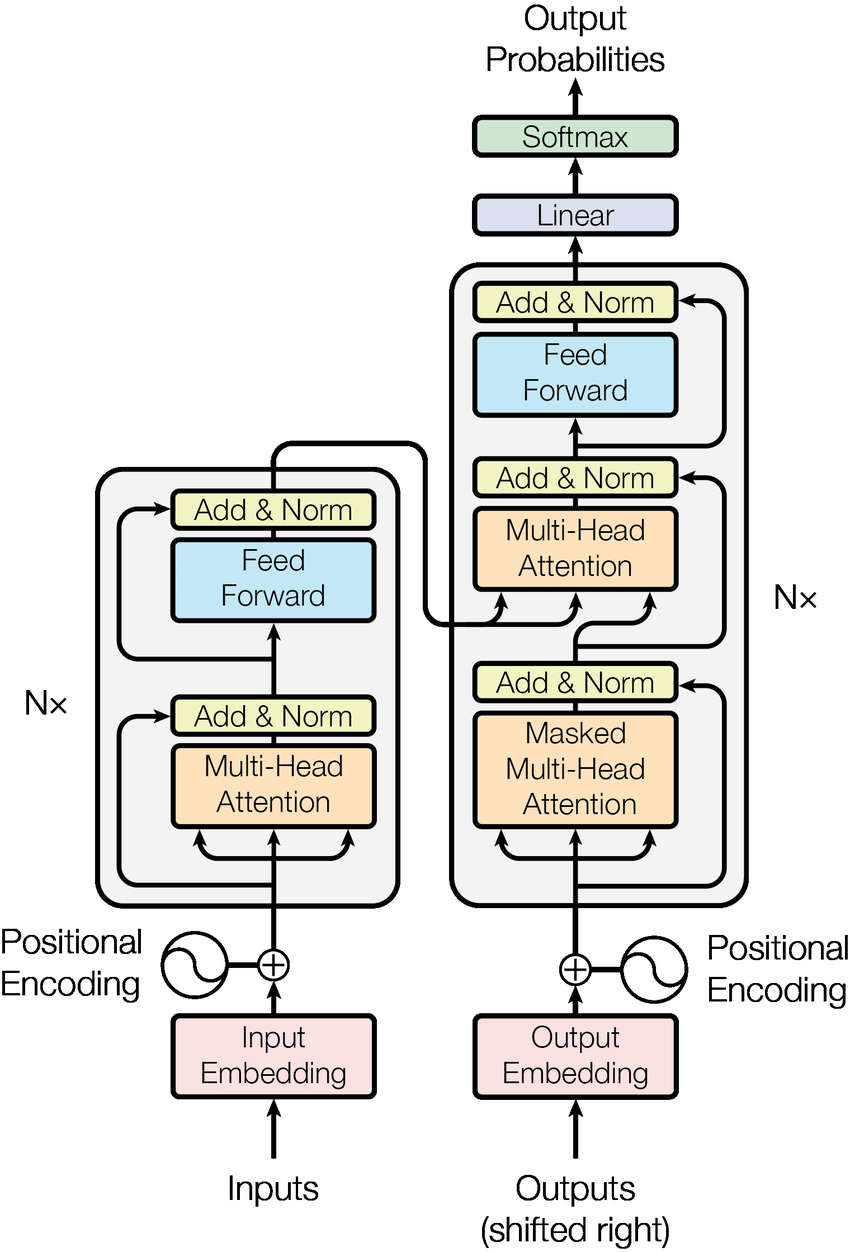
\includegraphics[width=.4\textwidth]{learners-overview/figure/transformer.png} \\
  \tiny{Transformer network architecture}
\end{center}
\end{minipage}

\end{frame}

% ------------------------------------------------------------------------------

\begin{frame}{Neural Networks -- method summary}

\footnotesize


\highlight{Hyperparameters}

\begin{itemize}
  \item \textbf{Architecture}:
  \begin{itemize}
    \item Lots of design choices $\Rightarrow$ tuning problem of its own.
    \item Typically: hierachical optimization of components (cells) and macro structure of network\\ 
    $\rightarrow$ \textbf{Neural Architecture Search (NAS)}
    \item Many predifined (well working) architectures exist for standard tasks
  \end{itemize}
  \item \textbf{Training}:
  \begin{itemize}
    \item Initial learning rate and various regularization parameters
    \item Number of epochs is determined by \textbf{early-stopping}
    \item \textbf{Data-augmentation}, e.g., applying random rotations to input images
    %Crucial due to \textbf{overparameterization} and strong 
    %\textbf{nonconvexity} 
    %\item E.g., weight initialization, choice of optimizer, learning rate, 
    %batch size, number of epochs, \dots
  \end{itemize}
\end{itemize}

\medskip

\highlight{Foundation models}

\begin{itemize}
    \item \textbf{Enormous} models trained on vast amounts of (general) data, e.g., all of wikipedia, in \textbf{self-supervised} fashion
    \item Used as starting point (\textbf{pre-trained}) and fine-tuned via \textbf{transfer} or \textbf{few-shot} learning for other tasks requiring little data
    \item Examples: GPT-3 for language, CLIP for vision-language, \dots
\end{itemize}

%\begin{itemize}
%    \item Makes choice of the architecture dispensable\\
%          $\Rightarrow$ Pre-defined architecture with pre-trained weights is used
%    \item Reduces training cost a lot, since pre-trained weights are only adapted during fine-tuning
%    \item \textbf{Pre-training} done in a self-supervised fashion on ubiquituous amount of data\\
%          $\Rightarrow$ In self-supervised learning, labels are generated from the data itself, no human labeling effort needed
%\end{itemize}

% \highlight{Runtime behavior} ~~ \textcolor{blue}{???}

\end{frame}


% ------------------------------------------------------------------------------

\begin{frame}{Neural Networks -- Implementation \& Practical hints}

\highlight{General hints}
\begin{itemize}
    \item Instead of NAS, use a standard architecture and tune training hyperparameters
    \item Training pipeline (data-augmentation, training schedules, ...) is more crucial than the specific architecture
    \item While NNets are state-of-the-art for \textbf{computer vision (CV)} and \textbf{natural language processing (NLP)}, we recommend not to use them for tabular data because alternatives perform better
    \item Computational efforts for training (and inference) can be very high, requiring specific hardware.\\
    $\rightarrow$ Using a service (esp. for foundation models) can be more cost efficient
\end{itemize}

%\highlight{Some options for regularization} 
%\begin{itemize}
%  \item Control weight magnitude with \textbf{weight decay} (L2 
%  regularization)
%  \item Interrupt training when validation error starts to pick up 
%  $\Rightarrow$ \textbf{early stopping}
%  \item Use \textbf{dropout} to deactivate neurons at random, thus down-sizing 
%  network
%  \item Expand training data and enforce invariances via \textbf{augmentation}
%  \item \dots
%\end{itemize}

%\highlight{Optimization tricks}
%\begin{itemize}
%  \item Accelerate training via optimizer (ADAM, Momentum)
%  \item Control learning rate with \textbf{schedulers}, or keep it 
%  \textbf{adaptive}
%  \item Use \textbf{batch normalization} for stability by keeping input distributions fixed throughout transformations
%  \item \dots
%\end{itemize}

% \highlight{Types of neural networks (RNNs, CNNs)}
% 
% \begin{itemize}
%   \item \textbf{Recurrent neural networks (RNNs}: Deep NN that make use of 
%   \textbf{sequential} information with temporal \textbf{dependencies} \\
%   $\rightarrow$ Frequently applied to \textbf{natural language processing}
%   \item \textbf{Convolutional neural networks (CNNs)}: Regularized version of the 
%   fully connected feed-forward NN (where each neuron is connected to all 
%   neurons of the subsequent layer) that abstracts inputs to feature maps via 
%   \textbf{convolution} \\
%   $\rightarrow$ Frequently applied to \textbf{image recognition}
% 
% \end{itemize}
% 
% \medskip
% 
% \highlight{Problem of neural architecture search (NAS)}
% 
% NN are \textbf{not off-the-shelf} methods -- the network architecture needs to 
% be tailored to each problem anew \\
% $\rightarrow$ Automated machine learning attempts to learn architectures

\medskip
 
\highlight{Implementation}

\begin{itemize}
  \item \textbf{R:} Use python libraries (below) via \texttt{reticulate}, but not really recommended except for toy applications.
  \item \textbf{Python libraries:} 
  \begin{itemize}
      \item \texttt{keras} for simple high level API 
      \item \texttt{PyTorch} for flexible design with a focus on research
      \item \texttt{TensorFlow} for flexible design with a focus on deployment / industry
      \item \texttt{huggingface} for pre-trained / foundation models
  \end{itemize}
\end{itemize}

\end{frame}


% ------------------------------------------------------------------------------

\begin{frame}{Neural Networks -- Pros \& Cons}

\footnotesize

\begin{columns}[onlytextwidth]
  \begin{column}{0.5\textwidth}
    \highlight{Advantages}
    \footnotesize
    \begin{itemize}
      \positem Applicable to \textbf{complex, nonlinear} problems
      \positem Very \textbf{versatile} w.r.t. architectures
      \positem State-of-the-art for CV and NLP
      \positem Strong \textbf{performance} if done right
      \positem Built-in \textbf{feature extraction}, obtained by intermediate
      representations
      \positem Easy handling of \textbf{high-dimensional} data
      \positem \textbf{Parallelizable} training 
    \end{itemize}
  \end{column}

  \begin{column}{0.5\textwidth}
    \highlight{Disadvantages}
    \footnotesize
    \begin{itemize}
      \negitem Typically, high computational \textbf{cost}
      \negitem High demand for \textbf{training data} 
      \negitem Strong tendency to \textbf{overfit}
      \negitem Requiring lots of \textbf{tuning expertise} 
      \negitem \textbf{Black-box} model -- hard to interpret or explain
    \end{itemize}
  \end{column}
\end{columns}

\end{frame}